\section{Vecindad basada en soluciones activas}
Esta vecindad surge del cambio de representación propuesto. En cada paso del algoritmo para construir una solución activa se consideran varias 
operaciones que <<compiten>> para ser planificadas (i.e. son planificables en ese momento) de las cuales se elige la que tiene la llave de mayor valor numérico. 

La idea es construir la vecindad a partir de estas operaciones que compiten. En un principio puede pensarse en considerar todos los posibles ordenamientos 
posibles para dichas operaciones pero esto da lugar a una vecindad demasiado grande por lo que se considera únicamente hacer cambios por pares de llaves 
entre la operación elegida y todas sus competidoras.

\begin{figure}[H]
\centering
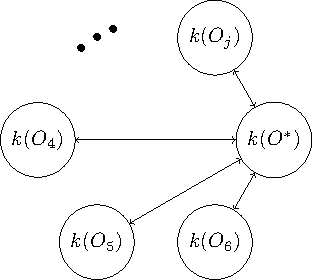
\includegraphics[scale=1.3]{Imagenes/vec2.pdf}
\caption{Movimientos de la vecindad propuesta. $k(O^*)$ es la llave de la operación elegida, las flechas representan los posibles intercambios entre las $j$ operaciones competidoras.}
\end{figure}
%diagrama

El tamaño de esta vecindad puede ser bastante grande ya que para cada paso del algoritmo \ref{alg:GT} se tienen tantos movimientos como operaciones competidoras, 
las cuales pueden ir desde 1 hasta el número de trabajos $n$ siendo en el peor caso de tamaño $O(nm*n)$. 
%
Como se mostrará mas adelante en la validación experimental, en realidad el número de operaciones que compiten por lo general es solo una fracción pequeña de $n$ 
con lo que la vecindad puede manejarse sin problemas.


Los movimientos de esta vecindad pueden generar soluciones muy diferentes dependiendo de dónde se encuentren en la planificación las operaciones consideradas. 
%
Si se cambia la llave de una operación que fue planificada al principio puede ser que la solución cambie en muchos otros lugares porque el conjunto de operaciones 
disponibles puede llegar a ser completamente distinto al llegar a un paso más avanzado en la construcción de la solución. 
%
Estas ideas podrían dar lugar a esquemas de reducción de vecindad, tratando de eliminar cambios que sean muy disruptivos;
%
sin embargo, dado que las vecindades que surgen para los casos tratados no son demasiados grandes se manejó la vecindad de forma completa.

\section{Extensión a vecindad N7}

Puesto que cada vez tenemos a nuestra disposición más recursos computacionales como punto de partida se planteó agregar movimientos a la vecindad N7 
con la cual se han obtenido los resultados del estado del arte.
%
Los movimientos que plantea esta vecindad solo tienen que ver con pares de operaciones en la ruta crítica por lo que una extensión sencilla consiste en 
considerar movimientos de operaciones que pueden no pertenecer a la ruta crítica. 

Es importante resaltar que si no se planteara también una función de fitness que no tome solo en cuenta el makespan estos movimientos nunca llevarían 
a una mejora \cite{blazewicz1996job}.
%
Los movimientos planteados se basan en observar que en alguna solución encontrada por una búsqueda local para cada máquina pueden existir periodos de tiempo en la 
que está inactiva (huecos) pero existe alguna operación en la ruta critica que podría comenzar a procesarse en este periodo y que se procesa después. 
%
Ninguna de las vecindades previamente propuestas considera movimientos de las operaciones de la ruta crítica más allá del bloque crítico por lo que estos movimientos 
representan un conjunto previamente no explorado de soluciones.

Intuitivamente lo que se pretende es llenar un hueco en la planificación con una operación de un bloque crítico.

\begin{figure}[H]
\centering
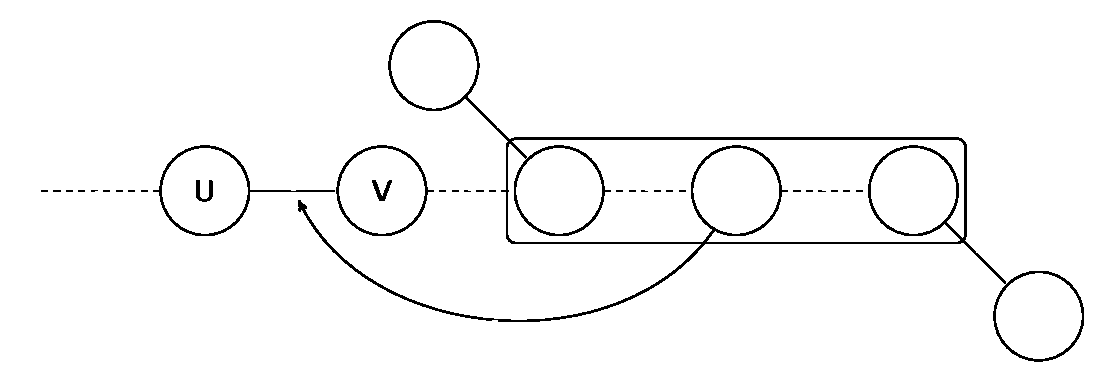
\includegraphics[scale=.7]{Imagenes/N8.pdf}
    \caption{Movimientos propuestos. El tiempo de inicio de \textbf{v} es mayor al de finalización de \textbf{u}}
\end{figure}

En general esta vecindad no extiende el número de vecinos visitados en una gran cantidad porque existen muchos de estos movimientos que hacen que la solución 
resultante sea infactible. 
